% THIS IS AN EXAMPLE DOCUMENT FOR VLDB 2012
% based on ACM SIGPROC-SP.TEX VERSION 2.7
% Modified by  Gerald Weber <gerald@cs.auckland.ac.nz>
% Removed the requirement to include *bbl file in here. (AhmetSacan, Sep2012)
% Fixed the equation on page 3 to prevent line overflow. (AhmetSacan, Sep2012)

\documentclass{vldb}
\usepackage{graphicx}
\usepackage{pgfplots}
\usepackage{balance}  % for  \balance command ON LAST PAGE  (only there!)

% Include information below and uncomment for camera ready
\vldbTitle{TLA+ Trace Checking In Production}
\vldbAuthors{A. Jesse Jiryu Davis, Judah Schvimer}
\vldbDOI{https://doi.org/10.14778/xxxxxxx.xxxxxxx}
\vldbVolume{12}
\vldbNumber{xxx}
\vldbYear{2019}

\begin{document}

% ****************** TITLE ****************************************

\title{TLA+ Trace Checking In Production}

% possible, but not really needed or used for PVLDB:
%\subtitle{[Extended Abstract]
%\titlenote{A full version of this paper is available as\textit{Author's Guide to Preparing ACM SIG Proceedings Using \LaTeX$2_\epsilon$\ and BibTeX} at \texttt{www.acm.org/eaddress.htm}}}

% ****************** AUTHORS **************************************

% You need the command \numberofauthors to handle the 'placement
% and alignment' of the authors beneath the title.
%
% For aesthetic reasons, we recommend 'three authors at a time'
% i.e. three 'name/affiliation blocks' be placed beneath the title.
%
% NOTE: You are NOT restricted in how many 'rows' of
% "name/affiliations" may appear. We just ask that you restrict
% the number of 'columns' to three.
%
% Because of the available 'opening page real-estate'
% we ask you to refrain from putting more than six authors
% (two rows with three columns) beneath the article title.
% More than six makes the first-page appear very cluttered indeed.
%
% Use the \alignauthor commands to handle the names
% and affiliations for an 'aesthetic maximum' of six authors.
% Add names, affiliations, addresses for
% the seventh etc. author(s) as the argument for the
% \additionalauthors command.
% These 'additional authors' will be output/set for you
% without further effort on your part as the last section in
% the body of your article BEFORE References or any Appendices.

\numberofauthors{2} %  
\author{
% The command \alignauthor (no curly braces needed) should
% precede each author name, affiliation/snail-mail address and
% e-mail address. Additionally, tag each line of
% affiliation/address with \affaddr, and tag the
% e-mail address with \email.
%
% TODO: don't repeat mailing address
% 1st. author
\alignauthor
A. Jesse Jiryu Davis\\
       \affaddr{MongoDB, Inc.}\\
       \affaddr{1633 Broadway}\\
       \affaddr{New York, NY 10019}\\
       \email{jesse@mongodb.com}
% 2nd. author
\alignauthor
Judah Schvimer\\
       \affaddr{MongoDB, Inc.}\\
       \affaddr{1633 Broadway}\\
       \affaddr{New York, NY 10019}\\
       \email{judah@mongodb.com}
}
% There's nothing stopping you putting the seventh, eighth, etc.
% author on the opening page (as the 'third row') but we ask,
% for aesthetic reasons that you place these 'additional authors'
% in the \additional authors block, viz.

% Just remember to make sure that the TOTAL number of authors
% is the number that will appear on the first page PLUS the
% number that will appear in the \additionalauthors section.


\maketitle

\begin{abstract}
We have multiple TLA+ specs to model various aspects of MongoDB. We use model-based trace-checking to test that real MongoDB replica sets' behaviors conform to these specs.
We apply the trace-checking technique to execution traces from fuzz tests, and deploy this system to our continuous integration infrastructure.
These tests continuously check for implementation behaviors that diverge from our specifications.
They allow us to simultaneously develop the implementation and specifications while staying reasonably confident that they conform.
Developing several specs and the implementation while maintaining a trace-checker is a challenge that the formal specification literature mostly omits, we describe some best practices.
\end{abstract}

\section{Introduction}

Formal modelling catches bugs \cite{Newcombe2014UseOfFormalMethodsAmazon}, but software engineers in industry are often skeptical of the value of the specification unless it can be shown to match the implementation \cite{Wayne18AgileFormalMethods, Newcombe2014UseOfFormalMethodsAmazon}, due to the risk of \textit{transcription bugs}. 
Further, it can be difficult to ensure that in a large engineering organization, changes in the production code are accompanied by changes in the specification of the code.
Nevertheless, formal methods are now being used to gain confidence in mission-critical, highly complex systems in multiple domains across many companies \cite{Tasiran03AlphaMicroprocessor}. 
Amazon \cite{Newcombe2014UseOfFormalMethodsAmazon, Chudnov18AmazonS2N, Cook18SecurityAWS}, Intel \cite{Kaivola09IntelI7, Beers08IntelExperience}, Microsoft \cite{Shukla18AzureCosmosDB}, and Springer \cite{Neubauer12AutomatedContinuousQualityAssurance}, have all written about their uses of formal methods and the value they've gained from using them to verify industrial software. 
Formal methods give confidence by covering every possible behavior within a given specification \cite{Kaivola09IntelI7}. 
They can expedite design of new features and confirm that a given solution fixes a bug. 
Specifications can allow engineers to make riskier change with less fear of dangerous bugs and can make a system more understandable by distilling away unnecessary complexity  \cite{Newcombe2014UseOfFormalMethodsAmazon}.

MongoDB has now used formal methods, specifically TLA+, for multiple projects on multiple teams. 
TLA+ has helped reproduce bugs found in tests and validate fixes for those bugs. 
MongoDB's replication protocol has especially gained from TLA+, verifying liveness properties of the database. 
It is impossible for a finite test to give confidence that a behavior will eventually, or never, happen. TLA+ has filled this gap, verifying protocols as safe that proved difficult to fix after numerous attempts \cite{Schultz19BugsLife}. 
Since this experience we have designed full features with their safety arguments grounded in TLA+ specs. 

We attempted to use model-based trace-checking (MBTC) \cite{MBTC} to gain confidence that our multiple TLA+ specifications match the C++ implementation of our distributed database, MongoDB.
Our proposed testing method would apply MBTC to execution traces obtained from our existing tests, and we would deploy our testing system to a cluster of continuous integration servers.
This would permit us to rapidly develop both the specifications and the implementation, while receiving quick feedback about divergences between the two \cite{Gravell11ConcurrentDevelopmentOfModelAndImplementation}.

We believe there are \textit{four requirements} for demonstrating "MBTC in production":
\begin{enumerate}
\item the implementation is a complex commercial software system
\item multiple specifications model aspects of the same system
\item the specifications and implementation co-evolve
\item the implementation's conformance to its specifications is continuously tested
\end{enumerate}

% TODO: some argument here or in another section about why these are required

We attempted to meet these four requirements, but hit multiple obstacles and ultimately found our direction impractical and we chose to abort our attempt.
In this paper we propose a vision for future research to make MBTC in production practical for systems like MongoDB.

This paper will provide a background to this research in Section \ref{sec:background}. Section \ref{sec:related_work} will review related work. Section \ref{sec:problem_statement} will identify the problem this work, and the future work it envisions, attempts to solve. Section \ref{sec:solution} describes the solution we attempted. Section \ref{sec:analysis} analyzes the challenges met in implementing the solution. Finally, Section \ref{sec:conclusions} details where this work left off and avenues for future work to make this approach more feasible in the future.

\section{Background}
\label{sec:background}


\section{Related Work}
\label{sec:related_work}

Our work builds primarily on the "eXtreme Modelling" approach proposed by Gravell, et. al. \cite{Gravell11ConcurrentDevelopmentOfModelAndImplementation}, which includes three characteristics:

\begin{enumerate}
\item The specifications and implementation co-evolve.
\item Multiple specifications model aspects of the system.
\item The implementation's conformance to its specifications is continuously tested.
\end{enumerate}

% In related work by Augusto, et. al.\cite{Augusto03ValidatingBusinessSystems}, the authors discusses the co-evolution of a Java implementation with several small specifications written in Promela and B.
% They describe specification engineering techniques; for example, holding regular meetings between specifiers and implementers, and maintaining a dictionary to translate between names in the specification and the implementation.
% Such engineering techniques seem promising, but the authors analyze their effectiveness when practiced on an example application developed by a team of four academics, not on commercial software developed by hundreds of engineers.

We have attempted to put the eXtreme Modelling ideas into practice with complex commercial software instead of a research prototype, and using TLA+ and C++ instead of Java, B, and Promela. To our knowledge, no prior research demonstrates all three characteristics of eXtreme Modelling in industry.

A variety of methods have been proposed to ensure that an implementation conforms to its formal specification.
Some projects use the same language for spec and implementation\cite{KerGre99},
or generate implementation code from the spec\cite{Houhou17CodeGenerationFromSpecification},
or apply model-checking or formal verification directly to the implementation\cite{Holzmann04ModelDrivenVerification},
or perform verified stepwise refinement from the high-level spec all the way down to the implementation\cite{Eiriksson95UsingFormalVerification}.
Any of these methods provides high confidence that the implementation conforms (although even a verified system is not bug-free \cite{Fonseca17EmpiricalStudy}). 
However, these methods cannot be used with our system, MongoDB.
In the research we have reviewed, they are limited to small programs written in C, or to specialized languages such as Prolog; they have not been demonstrated with our implementation language, C++, or other languages popular for large systems, such as Java.
They cannot be used when writing new specifications for a system that has already been implemented.

The "eXtreme Modelling" approach includes two testing methods that are promising for MongoDB: model-based testing\cite{Utting06PracticalModelBasedTesting} and model-based trace-checking\cite{Jard83AnApproachToTestingSpecifications, MBTC}. The former method uses the specification to generate test cases, either exhaustively or a carefully selected subset\cite{Dick93AutomatingGenerationOfTests}.
These tests exercise the implementation under test (IUT) to determine if it responds as specified to a variety of inputs.
In the latter, model-based trace-checking, the IUT is exercised with an integration test, random test, user test, or by observing its behavior in production.
The IUT produces an execution trace that captures its sequence of state changes.
This execution trace is checked against the model, either while the IUT is running or post-hoc, to verify that the trace is a permitted behavior of the specification.
The greater the variety of observed behaviors, the more confidence one has in the implementation's conformance.

Ural et. al. in \cite{Ural84AutomatedTestingOfProtocolSpecifications} propose to begin with a high-level specification and refine it in stages, using MBTC to gain confidence that each stage's model is equivalent to the previous stage.
Co-evolution of specification and implementation is not practical with this technique, because one would have to repeat the effort of stepwise refinement from top to bottom with each change, and it is unclear if multiple specifications could describe a single system.

% Tasiran et. al. \cite{Tasiran03AlphaMicroprocessor} implement MBTC to check that a simulated microprocessor's behavior conforms to its TLA+ specification.
% After each simulation step they invoke the TLC model-checker to determine if the step is permitted by the specification.
% The authors describe a sophisticated method to measure their tests' coverage of the specification's state space: they first eliminate symmetrical states, and project to a smaller space with a view function, before comparing to the covered space.
% They do not use multiple specifications, and there is no discussion of co-evolution of specification and implementation.

Neubauer et. al. in \cite{Neubauer12AutomatedContinuousQualityAssurance} use machine learning to infer a formal specification of a commercial software system from its observed behaviors.
They use MBTC to check if later execution traces of the system still conform to the inferred model; if not, either the system has a bug or the system behaved correctly and the model must be updated.
This work comes close to eXtreme Modelling, but an inferred specification is quite different from one written by humans; the purpose of the former is solely to detect behavior changes in the implementation, the latter expresses the designers' intent.

% TODO: Articles left to cite: \cite{Schultz19BugsLife, Schultz19TunableConsistency}

\section{Problem Statement}
\label{sec:problem_statement}

\section{Model-Based Testing}
\label{sec:model_based_testing}

Solution and analysis for Max's work

\section{Model-Based Trace-Checking}
\label{sec:model_based_trace_checking}

MongoDB database servers are typically deployed as a redundant group called a "replica set", which uses protocols inspired by Raft\cite{Ongaro14Raft} to elect a leader and replicate data changes to followers. Each replica stores a log of all operations (the "oplog"), a term counter that is incremented each election, and a timestamp representing the newest operation it knows has been committed by a majority of replicas (the "commit point"). We have written several TLA+ specifications to describe aspects of our protocol. Our goal was to test that a replica set's actual behavior conforms.

\subsection{Solution}

% 392 jstests in replsets/
% counting the following as "fuzz tests that exercise our replication protocol"
% initial_sync_multiversion_fuzzer_gen
% initial_sync_fuzzer_gen
% rollback_multiversion_fuzzer_gen
% rollback_fuzzer_gen
% rollback_fuzzer_clean_shutdowns_gen
% rollback_fuzzer_unclean_shutdowns_gen
% jstestfuzz_replication_continuous_stepdown_flow_control_gen
% jstestfuzz_replication_gen
% jstestfuzz_replication_multiversion_gen
% jstestfuzz_replication_initsync_gen
Prior to our research, there were roughly 400 integration tests handwritten in Javascript that exercise our replication protocol, and 10 fuzz tests that pause, disconnect, and terminate servers at random while the replica set is performing regular operations. We wanted to run these tests with additional trace logging, then use MBTC to check if the traces conform to our specifications.

% TODO: cite https://github.com/mongodb/mongo/blob/master/src/mongo/db/repl/tla_plus/RaftMongo/RaftMongo.tla
% Some say we should connect github.com/mongodb/mongo to Zenodo to get a DOI number, but that requires Office IT perms
% Uploading a repo snapshot to FigShare might be an easier way to get a DOI, or else just cite a URL with a commit hash
For our prototype we chose one of our specifications, a 345-line TLA+ file called \texttt{RaftMongo.tla}, which models the gossiping of the commit point among replicas. Each replica's state is modeled with four variables:

\begin{enumerate}
\item its role (leader or follower)
\item the newest election term it knows
\item the newest commit point it knows
\item the contents of its oplog
\end{enumerate}

There are seven named state transitions in the specification; they represent a write operation, an election, the replication of a data change, the gossipping of the commit point between replicas, and so on. 
% TODO: maybe more detail, or a diagram about RaftMongo.tla
% Counting commit f515d2ad which adds 275 lines, and rounding up because there were later adjustments
We located code paths in MongoDB corresponding to these seven state transitions and added logging statements, enabled only in testing, which emit as JSON the values of the four state variables above. The total code changes required approximately 300 lines of additional C++.

MBTC with a distributed system requires a partial order of trace events; we achieved a strict order by running all processes on one machine and adding millisecond sleeps where necessary while the system is under test. (Jard et. al. describe a solution with vector clocks \cite{Jard94GeneralApproachToTraceChecking}.)

% https://evergreen.mongodb.com/version/5e25ba97c9ec44650aa9944f
% replica_sets suite:
% https://evergreen.mongodb.com/task/mongodb_mongo_master_enterprise_rhel_62_64_bit_replica_sets_patch_fad0f06911036b04c5b40789d6ee5c58c4108f00_5e25ba97c9ec44650aa9944f_20_01_20_14_35_04
% 352 passed, 62 failed (presumably because they used arbiters or otherwise incompatible with trace logging)
% git clone https://github.com/will62794/faster-local-testing/
% python getlogs.py USER APIKEY --task mongodb_mongo_master_enterprise_rhel_62_64_bit_replica_sets_patch_fad0f06911036b04c5b40789d6ee5c58c4108f00_5e25ba97c9ec44650aa9944f_20_01_20_14_35_04

We enabled trace logging in Evergreen. This produced a total of TODO trace events in our handwritten Javascript tests on a particular run. We also selected one of our fuzz tests, called \texttt{rollback\_fuzzer}, for MBTC. This test randomly creates network partitions, causing replicas to temporarily diverge, then roll back writes in order to re-synchronize when the partitions are healed. A representative run of \texttt{rollback\_fuzzer} produced 2683 trace events.

% How much TLA+ statement and space coverage did today's rollback_fuzzer suite hit?
% from a given run of the suite, 1 JS file, 3 nodes, 2683 trace events
% Follow instructions on https://github.com/tlaplus/tlaplus/issues/413

% TODO: cite mongodb-labs/repl-trace-checker
We wrote a 484-line Python script to post-process trace logs. The script merges the replicas' logs and sorts them by timestamp to obtain a sequence of trace events. Each event describes only one replica's state at the moment it executed a state transition, from which the script must construct a sequence of states for the entire replica set. The script begins with a known initial state, combines it with the first trace event to determine the next state, and so on. For example, in Figure \ref{figure:event-processing}, the replica set's current state has Server 1 as the leader in term 1. The script processes a log message from Server 2 announcing it has become leader in term 2, arriving at the next state.

\begin{figure}
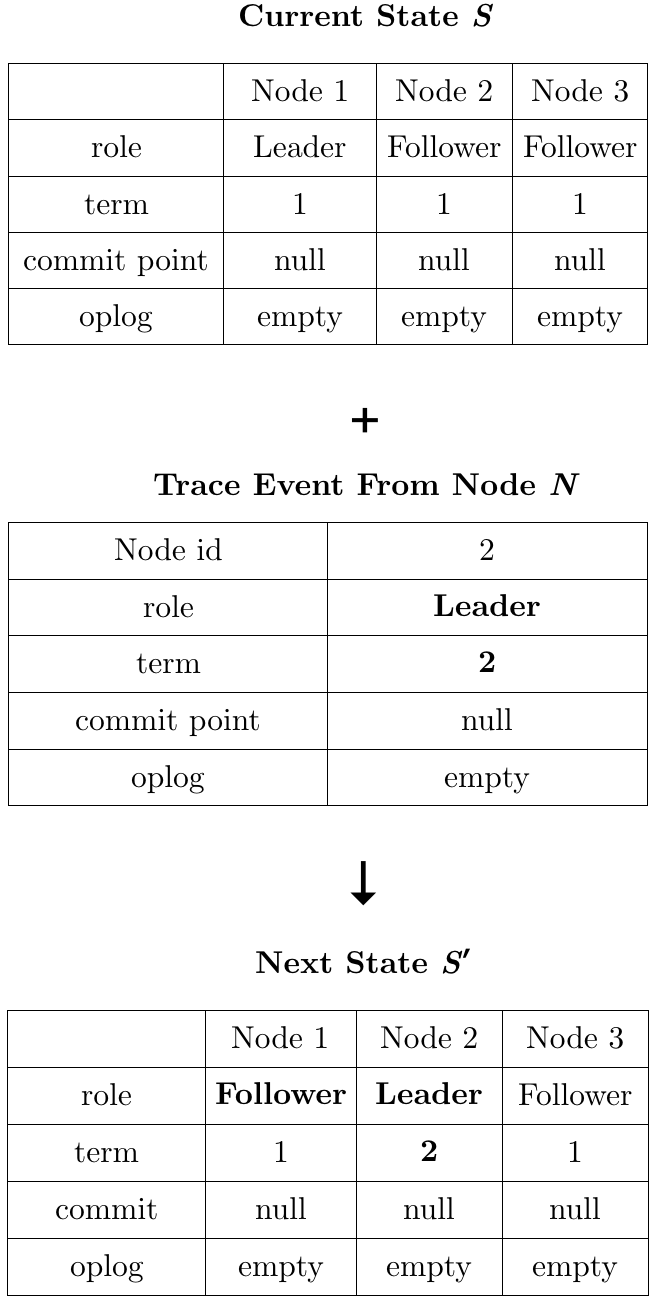
\includegraphics[width=8cm]{event-processing.png}
\caption{Trace Event Processing}
\label{figure:event-processing}
\end{figure}

Once the script has constructed this sequence of states, it implements MBTC following a method proposed by Pressler\cite{Pressler18VerifyingSoftwareTracesTLAPlus}: it generates a TLA+ module called \texttt{Trace.tla} which includes the sequence of states (Figure \ref{fig:state-sequence}), and uses the TLC model-checker to check that the sequence is permitted by the \texttt{RaftMongo.tla} specification.

\begin{figure}
\begin{verbatim}
------- MODULE Trace ------------
EXTENDS Integers, Sequences

\* Trace generated from replica set log files. Each
\* tuple is role, term, state, commit point, oplog
\* per server.

Trace == <<
<<
  <<"Leader", "Follower">>,
  <<1, 1>>,
  <<NULL, NULL>>,
  << <<>>, <<>> >>
>>,
<<
  <<"Follower", "Leader">>,
  <<1, 2>>,
  <<NULL, NULL>>,
  << <<>>, <<>> >>
>>
>>
\end{verbatim}
\caption{State sequence as TLA+ tuple (simplified)}
\label{fig:state-sequence}
\end{figure}

\subsection{Analysis}

% Probably irrelevant: We considered either a Java harness that fed trace inputs to the TLC internal API, and we tried Pressler's method. Since the former was not fully implemented in Java for us, and the latter already works and includes nice Toolbox diagnostics, we stuck w/ the latter. We also considered Pressler's suggestion of using his method w/ a custom operator that avoids passing through TLA+ tuples as the repr of the trace, we didn't need to do that either.

% Counting from Oct 10, 2019 https://github.com/mongodb-labs/repl-trace-checker/commit/5c96b44d to 
% Jan 10+.
We had intended to trace-check several specifications against traces from both handwritten and fuzz tests, deploy the trace-checker to our continuous integration system, and measure accumulated state space coverage over all tests. However, we applied trace-checking to only 5 handwritten tests and one fuzz test. Only one handwritten test generated traces that passed the trace-checker. We did not deploy to continuous integration nor measure coverage. The effort to implement MBTC proved so costly for us that we abandoned the project after two months of engineering effort. We faced discrepancies between our specifications and implementation, complexities with concurrency and locking, and incomplete support in TLC. In the following sections we describe these issues and propose future solutions.

\subsubsection{Implementation discrepancies}

% TODO: cite SERVER-17934

Trace checking the output of \texttt{rollback\_fuzzer} immediately reproduced a known violation of the specification: our implementation permits a new follower to commit oplog entries before it is fully synced with the leader, but this behavior should not be permitted, and is not modeled in \texttt{RaftMongo.tla}. This was not a \textit{transcription bug}; when we wrote \texttt{RaftMongo.tla} we did not have MBTC in mind, so we deliberately wrote an idealized spec. We intend to gradually bring our implementation into conformity. When MBTC caught this violation it increased our confidence in trace-checking. However, we needed some way to make the implementation pass trace checking. Since the violation came only 4 steps from the trace's start, and the checker stopped at the first violation, the violation left the remainder of the 2683 steps unchecked. To pass trace-checking, we could 1) update the specification to match today's implementation, 2) fix the implementation sooner than planned, 3) post-process the trace log to simulate a conformant implementation, or 4) avoid triggering the non-conforming behavior in testing. For this particular issue we chose solution 4, and modified \texttt{rollback\_fuzzer} to ensure all followers were fully synced before the test began any writes. However, we realized that updating all our fuzz tests and handwritten tests to avoid non-conforming behavior would not be economical, and would remove useful test coverage.

Other discrepancies required solution 1, updating the specification. For example, \texttt{RaftMongo.tla} modeled elections as an instantaneous change from one leader to another. This simplification was reasonable when the specification was first written, since the election protocol was not its original focus. But in fact elections comprise multiple events over time, and MBTC required us to make the specification more complex to account for this. Each discrepancy we discovered through MBTC required us to judge which of the four solutions was most cost-effective.

Lesson: In order to use a formal specification with MBTC, the specification should be written with MBTC in mind. We had started with specifications written for the sake of documenting and model-checking a design. If we started over, we would match our specifications to the known flaws in the implementation, and faithfully model multi-step events with multiple TLA+ actions.

\subsubsection{Hierarchical locking, visibility}

% Logging and locking, inter- vs intra-process concurrency. specs like Raft model inter proc concurrency but not intra proc. That seems true of the literature in general: one or the other kind of concurrency not both. We've found it hard to do MBTC for Raft because we have to make one process appear single-threaded so we can snapshot its state in the trace log, this is very hard in a highly concurrent process. This may be true of nearly all distributed systems in production.

% hierarchical locking is common to DBs (cite), but makes trace logging hard: at the layer being specified, must lock lower layers in order to get snapshot of system state for logging. this tends to contradict lock order rules. make a diagram!

% for each event, must log after event has changed process state, before the change is visible to any other process (or even thread in this process). essentially must take all locks and latches and stop the entire process, but a system designed for fine-grained hierarchical locking resists such an approach.

% oplog visibility - determining the moment in a process when its state can have an effect on other processes, better hope it's atomic or you must model both concurrencies in TLA+

Formal specifications of distributed systems algorithms, such as Raft, model a concurrent system of interacting processes, but they typically model each process as single-threaded. Production database systems such as MongoDB, however, almost always have high intra-process concurrency and employ some degree of hierarchical locking\cite{Gray76SharedLocks}. It may not be feasible to log a consistent snapshot of such a process's state at the moment of a trace event.

% _tlaPlusRaftMongoEvent_inlock's caller has replcoord mutex, the fn gets Global IS,
% DB IS, and Collection IS locks for local.oplog.rs.
% more details in https://mongodbcr.appspot.com/536420002/, particularly patch set 9
% map locks A, B, C to RSTL, Global, replcoord mutex.

For \texttt{RaftMongo.tla} specifically, a replica includes the contents of its oplog with each trace event. Acquiring the locks to obtain a snapshot of the oplog proved difficult. Suppose our \texttt{traceLogEvent} procedure (Figure \ref{fig:state-sequence}) must acquire locks A, B, and C, in that order, to read the oplog. Consider a procedure \texttt{becomeLeader} that acquires locks A and C, then changes the replica's role to Leader. If we add a call from \texttt{becomeLeader} to \texttt{traceLogEvent}, the latter must acquire lock B, but this is the wrong order and risks deadlocking with other threads.  General solutions are unpalatable: callers of \texttt{traceLogEvent} could be responsible for acquiring all the locks it will need, but this encodes intimate knowledge about \texttt{traceLogEvent} into its callers, and it significantly alters the system's behavior under test. Furthermore, MongoDB has no general Two-Phase Locking\cite{Eswaran76TwoPhaseLocking} framework, so such changes would be labor-intensive.

\begin{figure}
\begin{verbatim}
PROCEDURE becomeLeader() {
    acquire Lock A
    acquire Lock C
    role := Leader
    logTraceEvent()
}

PROCEDURE traceLogEvent() {
    /* Wrong acquisition order if called by
       becomeLeader, risks deadlock */
    acquire Lock A if not yet acquired
    acquire Lock B if not yet acquired
    acquire Lock C if not yet acquired
    read oplog
}
\end{verbatim}
\caption{Pseudocode for a replica becoming a Leader}
\label{fig:state-sequence}
\end{figure}

A related challenge is to log each trace event after it has occurred, but \textit{before} the change is visible to other replicas. E.g., when a leader appends an oplog entry, it must log the trace event after the entry has appeared in its own oplog, but before it can be replicated by any followers. If a follower logged a "Replicate Entry" event with an earlier timestamp than the leader's "Write Entry" event, the trace would violate the specification. We had to consider carefully when to log each trace event to achieve this fine timing.

Solving the two challenges above, for each of the seven named state transitions in \texttt{RaftMongo.tla}, was the single most difficult aspect of our MBTC implementation, costing more than a month of engineering effort. We discovered code locations that obeyed our visibility requirements, and managed to avoid the need for acquiring locks out of order by exploiting MongoDB's MVCC features instead. We expect any MBTC implementation for a concurrent database will encounter similar complexities with hierarchical locking and visibility of state changes.

If we began again, we would rewrite our specification to model events, such as protocol messages, that are easily observed in the implementation. We would avoid modeling state that is difficult to snapshot, especially if it is protected with complex locking. If some state in the model cannot be logged by the implementation, Pressler proposes a "refinement mapping" technique\cite{Pressler18VerifyingSoftwareTracesTLAPlus} that is worth further investigation.

\subsubsection{TLA+ and TLC}

% TODO: cite https://github.com/tlaplus/tlaplus/issues/413
Tool support for MBTC with TLA+ and TLC is a work in progress. Pressler's method works well to check traces of hundreds of events, but for thousands of events it is impractically slow. Pressler proposed, and Markus Kuppe has begun to implement, features to check long traces by bypassing the TLA+ parser in favor of a special-purpose Java extension to TLC. MBTC with TLA+ will be more convenient once these features are finalized and released, with several examples. Another missing feature is the ability to combine state-space coverage reports over multiple TLC executions, which would permit engineers to calculate the total coverage achieved by deploying MBTC to continuous integration.

% Debug failures with TLC output or exploration in TLA+ Toolbox GUI

% Estimates of effort, lines of code, MBTC runtime, other statistics


% It's nice to have spec and impl in one repo, and to add spec-specific tracing in the same commits as the spec & impl


% what does MBTC prove?
% Advantage of MBTC over other tests is that implementation tests can't prove liveness, unless you run them forever. TLA+ specs can be checked for liveness, and if the impl matches the spec, the impl might also not have liveness bugs.

% impl is a subset of the spec => if the spec is safe, the impl is safe
% but we can't test to the point where we know that impl is a subset of the spec
% we only know that tested behavior is a subset of the spec

% FALSE: impl is a subset of the spec => if the spec has no liveness bugs, the impl has no liveness bugs
% the impl might lack spec behaviors that are required for liveness

% use "refinement" jargon!

% Reconstruction of truncated oplogs

% Python performance was a bit challenging

% Choices about when to fix conformance in spec, MongoDB, or Python script

% Fixing spec can make it more complex and take longer to model-check and to read
% Might make some configs intractable to model-check that would've been tractable while the spec was more abstract

% the MBTC paper made it sound like adding trace logging was easy: they use AspectJ and other Java-specific tech to add fairly non-intrusive logging, with introspection to avoid writing a ton of code, and they don't discuss concurrency problems with getting a point-in-time snapshot of a single process's state. In our highly concurrent C++ application, which is very large and old and not written with MBTC in mind, we found trace logging to be the hardest(?) part to implement

\section{Conclusions}
\label{sec:conclusions}

And future work.

%\end{document}  % This is where a 'short' article might terminate

% ensure same length columns on last page (might need two sub-sequent latex runs)
\balance

%ACKNOWLEDGMENTS are optional
\section{Acknowledgments}
\label{sec:acknolwedgments}


% The following two commands are all you need in the
% initial runs of your .tex file to
% produce the bibliography for the citations in your paper.
\bibliographystyle{abbrv}
\bibliography{main}  % use main.bib file
% You must have a proper ".bib" file
%  and remember to run:
% latex bibtex latex latex
% to resolve all references
\end{document}
\balance
